\documentclass{article}
\usepackage{indentfirst}  % Adds indentation to the first paragraph of each section
\usepackage{amsmath}      % Provides additional math symbols
\usepackage{amssymb}      % Provides \mathbb for blackboard bold symbols
\usepackage{hyperref}     % For hyperlinks in the bibliography
\usepackage{stmaryrd}
\usepackage{tikz}
\usetikzlibrary{3d}
\usepackage{pgfplots}
\usepackage{tikz-3dplot}
\usepackage{graphicx}

\usepackage{caption}
\captionsetup{labelformat=empty}  % Removes "Figure X" from captions

\setlength{\parindent}{15pt}  % Adjust the size of the paragraph indent
\linespread{1.5}  % Set line spacing to 1.5 times

\begin{document}

\section*{\centering Chapter I}
\section*{\centering Application of the theory of conceptual spaces to colours}

\subsection*{1.1. From RGB to HSL}

\hspace*{\parindent}A colour space is used to represent the three-dimensional organisation of colours. Colours are mapped along axes that represent different colour properties. A first example is the space $\mathbf{RGB}$ whose three dimensions represent red, green, and blue respectively.

A singular colour shade is represented in $\mathbf{RGB}$ by a triplet\footnote{This space is often used in computing, where the value of red, green and blue is encoded by a byte that can have 256 different values.} $\left(x_1,x_2,x_3\right) \in \left(R \times G \times B\right)$ where $R \times G \times B = \llbracket 0 ; 255 \rrbracket \times \llbracket 0 ; 255 \rrbracket \times \llbracket 0 ; 255 \rrbracket \subset \mathbb{N}^3$. Intuitively, this triplet represents the level of red, green, and blue in the singular colour shade.

More generally, the $\mathbf{RGB}$ space models each colour shade as an additive combination of its value over the three dimensions of red, green, and blue. $\mathbf{RGB}$ space can be represented by a cube, where each axis represents the intensity of the components: red, green, and blue.

Although the \textbf{RGB} space has the merit of being simple, we will present two schematic ideas that show that it is not at all suitable for modelling human vision. Firstly, since the dimensions of \textbf{RGB} are chromatic, brightness information must be extracted from the three components encoding chromaticity. However, to model the human visual system, it is more appropriate to isolate a brightness parameter from the chromaticity parameters \cite[p.78]{fairchild2013}. The second criticism concerns the opposite colours in \textbf{RGB}. When space \textbf{RGB} is represented as a cube, it appears that each vertex — which intuitively corresponds to a 'pure colour' — has an opposite vertex that is also the furthest away on the cube. In other words, the four diagonals joining the four opposite vertices on the cube indicate the four pairs of colours furthest apart (cf. Fig. 1a). Thus, one of the shortcomings of the \textbf{RGB} model is that the vertex opposite that of RED is the one corresponding to CYAN. However, during the nineteenth and twentieth centuries, a number of empirical studies and theories\footnote{Based on psychophysical experiments, Hering (1834-1918) argued that carmine red is the opposite of green and that blue is the opposite of yellow. This idea gave rise to the opponent process theory, which states schematically that certain green stimuli and certain red stimuli generate opposite neurobiological responses (on the 3 types of rods: L; S; M) or even antagonistic (mutually incompatible) responses.} support the idea that the most opposite colour to RED is GREEN, and not CYAN as is the case in \textbf{RGB}.

Gärdenfors \cite[section 2.1]{gardenfors2014} presents the three-dimensional colour space \textbf{HSL}, comprising the dimensions of hue, saturation and luminosity. This model solves the two problems previously raised: firstly, it dissociates the luminosity dimension from the chromatic dimensions, and secondly, it separates RED and GREEN on the saturation axis as far as possible (see Fig. 1.b).

\begin{figure}[h]
\centering
\begin{minipage}[b]{0.45\textwidth}
\centering
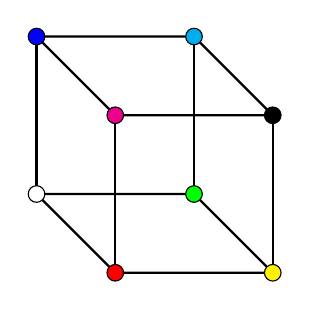
\begin{tikzpicture}[x={(0.5cm,-0.5cm)}, y={(1cm,0cm)}, z={(0cm,1cm)}]

% Define the coordinates of the cube
\coordinate (A) at (0,0,0);
\coordinate (B) at (2,0,0);
\coordinate (C) at (2,2,0);
\coordinate (D) at (0,2,0);
\coordinate (E) at (0,0,2);
\coordinate (F) at (2,0,2);
\coordinate (G) at (2,2,2);
\coordinate (H) at (0,2,2);

% Draw the back face
\draw[thick] (D) -- (C) -- (B) -- (A) -- cycle;

% Draw the front face
\draw[thick] (E) -- (F) -- (G) -- (H) -- cycle;

% Connect the front and back faces
\draw[thick] (A) -- (E);
\draw[thick] (B) -- (F);
\draw[thick] (C) -- (G);
\draw[thick] (D) -- (H);

% Add colored circles with black outlines at the vertices
\draw[black, fill=white] (A) circle (3pt);
\draw[black, fill=red] (B) circle (3pt);
\draw[black, fill=yellow] (C) circle (3pt);
\draw[black, fill=green] (D) circle (3pt);
\draw[black, fill=blue] (E) circle (3pt);
\draw[black, fill=magenta] (F) circle (3pt);
\draw[black, fill=black] (G) circle (3pt);
\draw[black, fill=cyan] (H) circle (3pt);

\end{tikzpicture}
\caption{Figure 1a. \textbf{RGB} Space}  % Custom caption text
\label{fig:rgb_cube}
\end{minipage}
\hfill
\begin{minipage}[b]{0.45\textwidth}
\centering
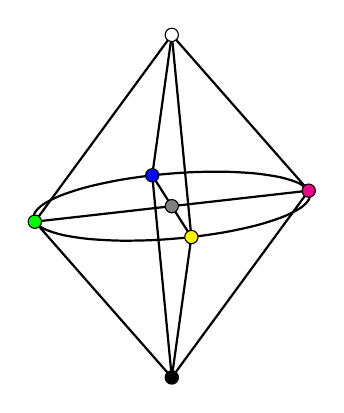
\begin{tikzpicture}[scale=1.2]  % Adjust the scale factor as needed
    % Set up a 3D coordinate system with more inclined viewing angles
    \tdplotsetmaincoords{115}{15}  % Adjust elevation to 115° and azimuth to 15° (slight X-axis rotation)
    \begin{scope}[tdplot_main_coords]

        % Vertices for the upper and lower points of the tetrahedron
        \coordinate (A) at (0,0,2);  % Top vertex (white)
        \coordinate (F) at (0,0,-2); % Bottom vertex (black)

        % Coordinates for the flat ellipse and colored points
        \coordinate (B) at (1.5,0,0);   % Right point on the X-axis (magenta)
        \coordinate (C) at (-1.5,0,0);  % Left point on the X-axis (green)
        \coordinate (G) at (0,0,0);     % Center point (grey)

        % Adjusted coordinates for yellow and blue points to lie on the ellipse
        \coordinate (D) at (0,0.8,0);     % Front point on the ellipse (yellow)
        \coordinate (E) at (0,-0.8,0);    % Back point on the ellipse (blue)

        % Draw the ellipse (thin, flat in the XY plane)
        \draw[thick] plot[smooth,domain=0:360]
            ({1.5*cos(\x)}, {0.8*sin(\x)}, 0); % Ellipse with 1*sin(\x) for the Y component

        % Draw the perpendicular diametric segments (X-axis and Z-axis)
        \draw[thick] (B) -- (C);  % X-axis segment (green-magenta)
        \draw[thick] (D) -- (E);  % Z-axis segment (yellow-blue)

        % Draw the edges connecting the top and bottom vertices to the points on the ellipse
        \draw[thick] (A) -- (B);
        \draw[thick] (A) -- (C);
        \draw[thick] (A) -- (D);
        \draw[thick] (A) -- (E);
        \draw[thick] (F) -- (B);
        \draw[thick] (F) -- (C);
        \draw[thick] (F) -- (D);
        \draw[thick] (F) -- (E);

        % Add the vertices as colored points
        \filldraw[fill=white, draw=black] (A) circle (2pt);  % top vertex (white)
        \filldraw[fill=black, draw=black] (F) circle (2pt);  % bottom vertex (black)
        \filldraw[fill=magenta, draw=black] (B) circle (2pt);  % right (magenta)
        \filldraw[fill=green, draw=black] (C) circle (2pt);  % left (green)
        \filldraw[fill=yellow, draw=black] (D) circle (2pt);  % front (yellow)
        \filldraw[fill=blue, draw=black] (E) circle (2pt);  % back (blue)
        \filldraw[fill=gray, draw=black] (G) circle (2pt);  % center (grey)

    \end{scope}
\end{tikzpicture}
\caption{Figure 1b. \textbf{HSL} Space}  % Custom caption text
\label{fig:tetrahedron}
\end{minipage}
\end{figure}

\subsection*{1.2. Using psychophysical experiments on human vision as a starting point}

The \textit{Commission internationale de l'éclairage} (CIE) is the institution in charge of standards for photometry and colorimetry. In 1976, the CIE recommended the use of \textbf{CIELAB} space to represent colours seen on paper or textiles, and \textbf{CIELUV} space to represent colours perceived on a screen. Since then, the \textbf{CIELAB} space has been adjusted, corrected and optimised, which is less the case with \textbf{CIELUV}, whose use has declined somewhat in favour of other spaces\footnote{Fairchild (2013, pp.313-316) reviews the conditions of several experiments in which \textbf{CIELAB} performed better than \textbf{CIELUV}. Among other things, he cites an experiment using pairwise comparisons of printed images in which \textbf{CIELAB}'s predictions were significantly better than those of \textbf{CIELUV} (\textit{Ibid}, p.313).}. To set up these colour spaces and the corresponding operations, the CIE first had to define certain \textit{psychophysical reference conditions}. These conditions are those of a "standard observer" who is used to \textit{standardise} the different results of observations, i.e. to interpret them under the same methodological standards. For example, one of the standards for colorimetric tests is the use of illuminant D65, which has been statistically defined from numerous measurements of daylight (Fairchild, 2013, p.62). In 'D65', the uppercase '\textit{D}' indicates that it is a daylight measurement ('Daylight') and the number indicates approximately the colour temperature\footnote{The temperature of D65 is 6504 Kelvin.}. Illuminant D65 is a slightly cool white that corresponds roughly to daylight in the northern hemisphere, under slightly cloudy skies, between 10am and 12pm in spring and autumn (Berns 2019, p.4; Hirsch, 2014, p.72). In addition to lighting, the reference  psychophysical conditions also include object modalities (e.g. \textit{fabric, paper, screen}), background colour or stimulus size in degrees of visual angle\footnote{In 1995, the CIE introduced a colour difference measurement called 'CIE94', whose reference conditions include a uniform background with a neutral grey (L = 50) and a visual angle greater than 4°, which refers roughly to the perceived size of a circle 3.5cm in diameter placed 50cm from an observer (Berns 2019, p.103; Fairchild 2013, p.83).}

Space \textbf{CIELAB} is defined in three dimensions \textit{〈L ;a ;b〉}. The \textit{a} axis represents saturation, the \textit{b} axis represents hue and the \textit{L} axis indicates the degree of luminosity. Thus, although the structure of the \textbf{CIELAB} and \textbf{CIELUV} spaces seem similar\footnote{On the precise differences between \textbf{CIELAB} and \textbf{CIELUV}, see (Fairchild, 2013, p.211).}



\bibliographystyle{plain}
\bibliography{references}

\end{document}
